\documentclass[11pt,letterpaper]{article}
\usepackage[margin=.72in]{geometry}
\usepackage[T1]{fontenc}
\usepackage{lmodern,microtype,booktabs,array,graphicx,pdflscape,xcolor,amsmath,hyperref}
\hypersetup{colorlinks=true,urlcolor=blue,linkcolor=blue,pdftitle={Reported injury rates depend on exposure}}
\setlength{\parindent}{0pt}\setlength{\parskip}{6pt}
\newcommand{\heading}[1]{\vspace{4pt}{\large\bfseries #1}\par}
\newcommand{\BoundA}{92.53}
\newcommand{\BoundB}{1}
\newcommand{\BoundC}{115,164}
\newcommand{\BoundD}{361,383,028,589}
\newcommand{\BoundE}{0.063735}
\newcommand{\BoundF}{400,288}
\newcommand{\BoundG}{46,530}
\newcommand{\BoundH}{46,511}
\newcommand{\BoundI}{19}
\newcommand{\BoundJ}{3,571}
\newcommand{\BoundK}{0}
\newcommand{\BoundL}{1,257}
\newcommand{\BoundM}{6,662}
\newcommand{\BoundN}{0.258}
\newcommand{\BoundO}{2,203}
\newcommand{\BoundP}{1}
\newcommand{\BoundQ}{194}
\newcommand{\BoundR}{13,386}
\newcommand{\BoundS}{0.268}
\newcommand{\BoundT}{476}
\newcommand{\BoundU}{0}
\newcommand{\BoundV}{135}
\newcommand{\BoundW}{1,211}
\newcommand{\BoundX}{2.908}
\newcommand{\BoundY}{9,637}
\newcommand{\BoundZ}{11}
\newcommand{\BoundAA}{3,754}
\newcommand{\BoundAB}{15,339}
\newcommand{\BoundAC}{2.423}
\newcommand{\BoundAD}{4,073}
\newcommand{\BoundAE}{2}
\newcommand{\BoundAF}{650}
\newcommand{\BoundAG}{17,060}
\newcommand{\BoundAH}{2.109}
\newcommand{\BoundAI}{2,961}
\newcommand{\BoundAJ}{1}
\newcommand{\BoundAK}{1,161}
\newcommand{\BoundAL}{5,536}
\newcommand{\BoundAM}{0.003}
\newcommand{\BoundAN}{13,654}
\newcommand{\BoundAO}{2}
\newcommand{\BoundAP}{5,515}
\newcommand{\BoundAQ}{22,368}
\newcommand{\BoundAR}{1.296}
\newcommand{\BoundAS}{6,122}
\newcommand{\BoundAT}{2}
\newcommand{\BoundAU}{1,000}
\newcommand{\BoundAV}{26,366}
\newcommand{\BoundAW}{2.160}
\newcommand{\BoundAX}{3,814}
\newcommand{\BoundAY}{0}
\newcommand{\BoundAZ}{1,551}
\newcommand{\BoundBA}{7,236}
\newcommand{\BoundBB}{1.958}
\newcommand{\BoundBC}{31,183}
\newcommand{\BoundBD}{0}
\newcommand{\BoundBE}{2}
\newcommand{\BoundBF}{55}
\newcommand{\BoundBG}{27}
\newcommand{\BoundBH}{135,204}
\newcommand{\BoundBI}{1}
\newcommand{\BoundBJ}{38.78}
\newcommand{\BoundBK}{221,241,028,589}
\newcommand{\BoundBL}{0.104}
\newcommand{\BoundBM}{1}
\newcommand{\BoundBN}{92.53}
\newcommand{\BoundBO}{26,984,308,589}
\newcommand{\BoundBP}{0.854}
\newcommand{\BoundBQ}{10}
\newcommand{\BoundBR}{95.86}
\newcommand{\BoundBS}{14,978,817,537}
\newcommand{\BoundBT}{1.538}
\newcommand{\BoundBU}{599}
\newcommand{\BoundBV}{97.83}
\newcommand{\BoundBW}{7,843,757,569}
\newcommand{\BoundBX}{2.921}
\newcommand{\BoundBY}{140,142,000,000}
\newcommand{\BoundBZ}{15,217}
\newcommand{\BoundCA}{445,371}
\newcommand{\BoundCB}{315,540}
\newcommand{\BoundCC}{1,004,148}
\newcommand{\BoundCD}{40}
\newcommand{\BoundCE}{21}
\newcommand{\BoundCF}{3.10.11}
\newcommand{\BoundCG}{3.12.14}
\newcommand{\BoundCH}{31}
\newcommand{\BoundCI}{62}
\newcommand{\BoundCJ}{248}
\begin{document}
{\LARGE\bfseries Reported injury rates depend on exposure\par}
\vspace{5pt}
Independent research program\hfill 31 October 2026 UTC\\
\textit{Not peer reviewed. Current submitted summary data; descriptive sensitivity.}

\heading{Practical finding}
A pooled injury rate can be dominated by a few reported exposure values. In this fixed manufacturing cohort, the five highest-hour records account for \BoundA{}\% of eligible reported hours, while carrying \BoundB{} reported case. This concentration audit is explicitly retrospective: it was added after the frozen comparison exposed the denominator imbalance.

The full eligible cohort reports \BoundC{} cases over \BoundD{} hours, a pooled rate of \BoundE{} per 100 full-time-equivalent worker-years. These are source-accounting values, not a validated population rate or evidence that the exposure values are correct. Both independent source parsers agree with the captured native values; that agreement does not establish source truth.

\heading{Recommended use}
Audit exposure concentration before using a pooled reported rate to center smoothing. A dashboard should retain the numerator, reported hours, missingness and smoothing assumptions. Seek source clarification for extreme exposure values before operational use. Do not silently cap or remove observations and call the result corrected.

The original source and all frozen estimates remain unchanged. Conditional rates after removing the highest-hour records are presented as accounting diagnostics, not cleaned estimates or a recommendation to delete those records. No employer identities or rankings are public.

\heading{Source and fixed scope}
The official OSHA 2025 Summary Data file contains \BoundF{} rows. The fixed cohort retains \BoundG{} manufacturing records in broad NAICS prefixes 31, 32 and 33 with reported maximum-size codes for 20--99, 100--249 or unsplit 20--249 employees. Annual average employment is not the size selector. \BoundH{} records have a consistent known numerator and positive reported hours; \BoundI{} nonpositive-hour records remain explicitly outside the rate denominator.

The numerical design was committed after the file was downloaded but before establishment values were parsed. Only the header, size and hash had been inspected. Values were visible during source reconciliation; this was source informed, not blinded. One current posted file does not establish original submission timing, physical-establishment identity or prediction-time availability.
\newpage
{\Large\bfseries Complete fixed accounts and conditional diagnostics\par}
{\small\setlength{\tabcolsep}{5pt}
\begin{tabular}{@{}llrrrrr@{}}\toprule
NAICS & Maximum size & Eligible & Excluded & Zero cases & Cases & Raw rate\\\midrule
31 & 20-99 & \BoundJ{} & \BoundK{} & \BoundL{} & \BoundM{} & \BoundN{} \\
31 & 100-249 & \BoundO{} & \BoundP{} & \BoundQ{} & \BoundR{} & \BoundS{} \\
31 & 20-249 unsplit & \BoundT{} & \BoundU{} & \BoundV{} & \BoundW{} & \BoundX{} \\
32 & 20-99 & \BoundY{} & \BoundZ{} & \BoundAA{} & \BoundAB{} & \BoundAC{} \\
32 & 100-249 & \BoundAD{} & \BoundAE{} & \BoundAF{} & \BoundAG{} & \BoundAH{} \\
32 & 20-249 unsplit & \BoundAI{} & \BoundAJ{} & \BoundAK{} & \BoundAL{} & \BoundAM{} \\
33 & 20-99 & \BoundAN{} & \BoundAO{} & \BoundAP{} & \BoundAQ{} & \BoundAR{} \\
33 & 100-249 & \BoundAS{} & \BoundAT{} & \BoundAU{} & \BoundAV{} & \BoundAW{} \\
33 & 20-249 unsplit & \BoundAX{} & \BoundAY{} & \BoundAZ{} & \BoundBA{} & \BoundBB{} \\
\bottomrule\end{tabular}}

Rates are reported cases per 100 full-time-equivalent worker-years, using 200,000 hours. Every fixed stratum is retained, including the unsplit legacy size class. NAICS versions can differ. Source-account categories, exact exposures and rates remain in the complete exports; no annual-average substitution or missing-to-zero fill is used.

\heading{All declared descriptive shrinkage strengths}
Let $t=h/200{,}000$ and $\mu=\sum k/\sum t$ across the complete eligible cohort. A Gamma--Poisson working model uses Gamma shape $b\mu$ and rate $b$, giving mean $(k+b\mu)/(t+b)$. The fixed prior exposures $b\in\{0.1,1,10\}$ span 20,000--2,000,000 hours. They are authored sensitivity probes, not tuned or empirically validated defaults. The center is estimated from this same cohort.

The authored boundary is rate $>2\mu$, with no regulatory or safety meaning. The raw rate exceeds it for \BoundBC{} records. At $b=0.1,1,10$, respectively, \BoundBD{}, \BoundBE{} and \BoundBF{} move to at/below the boundary; none moves upward. All \BoundBG{} stratum/strength accounts and \BoundBH{} sufficient-cell/strength cases are exported. No winner is selected and no future accuracy is measured.

\heading{Retrospective concentration audit: all four cases}
{\small\setlength{\tabcolsep}{6pt}
\begin{tabular}{@{}rrrrr@{}}\toprule
Top records & Top cases & Hours share & Remaining hours & Conditional rate\\\midrule
1 & \BoundBI{} & \BoundBJ{}\% & \BoundBK{} & \BoundBL{} \\
5 & \BoundBM{} & \BoundBN{}\% & \BoundBO{} & \BoundBP{} \\
10 & \BoundBQ{} & \BoundBR{}\% & \BoundBS{} & \BoundBT{} \\
100 & \BoundBU{} & \BoundBV{}\% & \BoundBW{} & \BoundBX{} \\
\bottomrule\end{tabular}}

All four conditional rates use the remaining submitted records. They are retrospective diagnostics, not replacement population estimates. The largest single reported exposure is \BoundBY{} hours. No source error is asserted without clarification.

For zero recorded cases, $-\log(0.05)/t$ is the one-sided 95\% upper rate under a homogeneous independent Poisson process. All \BoundBZ{} zero-case records and complete stratum bounds are retained. This assumption-based illustration has no measured interval calibration or workplace-safety validity.
\newpage
{\Large\bfseries Verification, implementation and limits\par}
\heading{Independent evidence}
Separate pandas C parsing, SQLite key multiplicities and exact Fraction tokens reconcile all native rows in \BoundCA{} finite conditions. Saved native-bound source checks pass \BoundCB{}. Independent weighted SQLite and exact-rational reconstruction checks every account, cell/strength, strict boundary, switch direction and request in \BoundCC{} conditions. The retrospective record-expanded SQLite concentration audit passes \BoundCD{} conditions.

The original committed freeze bound \BoundCE{} actual dependencies before comparisons. A disclosed post-analysis gzip-container amendment changes one writer, preserving every numeric result and the original code/freeze in HISTORY. Byte-preserving Git checkout fixes an inherited Windows line-ending failure. Both isolated full-history CPython \BoundCF{} and \BoundCG{} replays reproduce six files exactly, with all six source-directory files unchanged. Failed compatibility evidence is retained.

All \BoundCH{} authored fixture methods pass, covering maximum versus average employment, documented injury-flag codes, duplicate groups, missing/invalid counts, zero/nonpositive hours, exact rate ties, prior strengths and unsupported inferences. The inspected figures bind \BoundCI{} actual SVG bars and \BoundCJ{} coordinate conditions. Finite checks are not universal correctness guarantees.

\heading{Runnable implementation exercise}
Seven requests return two qualified reported-stratum accounts and reject safety ranking, legal fault, worker eligibility, future risk and denominator substitution. The interface retains numerator, exposure and explicit unknown safety/future accuracy. It does not certify arbitrary caller data or a production service.
\begin{verbatim}
python -m pip install -r requirements.txt
python src/replay.py --out ../injury-rate-replay
python src/check_diagnostics.py
\end{verbatim}
Use a new output directory. The replay uses saved counts; it does not redownload mutable native data.

\heading{Material limits and next evidence}
The original year-held-out partial-pooling proposal remains unexecuted. This is a same-cohort-centered descriptive sensitivity study, with no protected test, future-risk accuracy or new estimator. Source reporting, optional/nonrequired submissions, mixed industry-code versions and unknown physical-establishment identity limit generalization. Reporting does not establish fault, violation or benefit eligibility. No causal, production-use or realized-savings claim is made.

Raw establishment names, addresses, EINs, identifiers and native files remain private. No case-detail or worker data were requested. Separate formal-publication projects, including Azure optimization, remain private. Seek corrected or clarified exposure and verified identity/dated availability before a predictive extension.

{\small Source: OSHA Injury Tracking Application, 2025 Summary Data, submitted January--August 2026, captured 31 October 2026 UTC.
\url{https://www.osha.gov/itadata}.
Definitions: April 2024 Summary Data Dictionary and January 2025 ITA Data Users Guide. Exact URL, native hash, source accounts and earlier access failures are retained. OSHA does not endorse this independent analysis. MIT covers original code; government facts are attributed separately.}
\begin{landscape}
{\large\bfseries Retrospective exposure concentration\par}
\begin{center}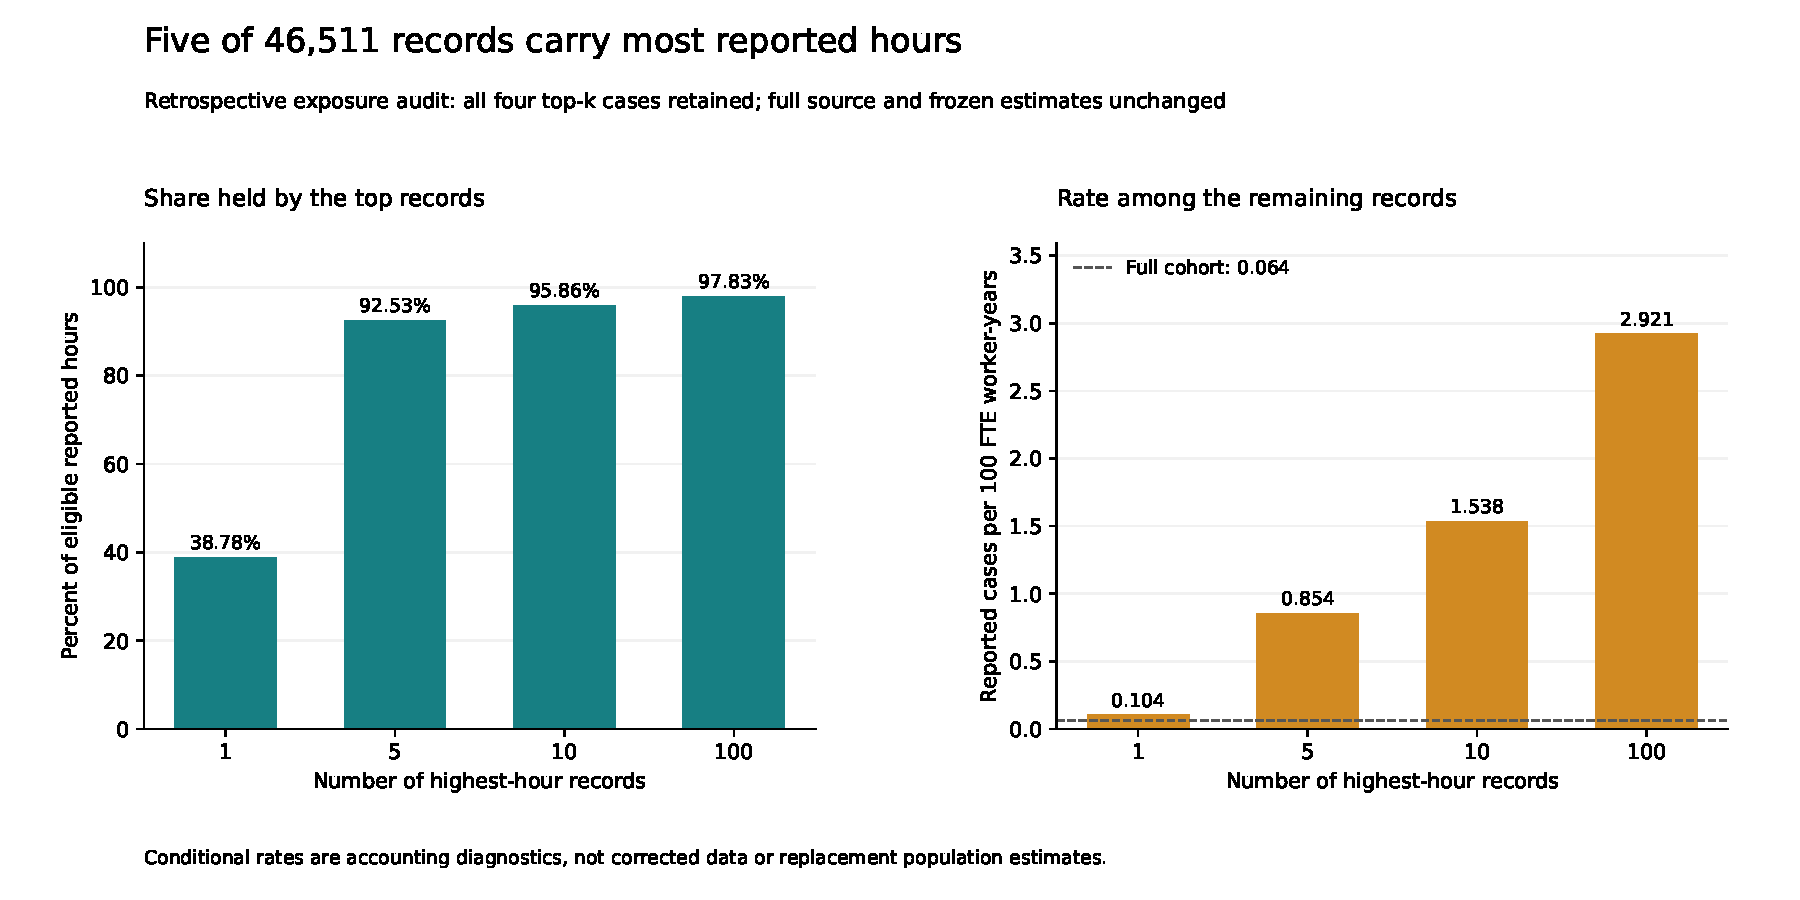
\includegraphics[width=9.4in,height=6.25in,keepaspectratio]{images/exposure_concentration.pdf}\end{center}
\end{landscape}
\begin{landscape}
{\large\bfseries Complete declared smoothing comparisons\par}
\begin{center}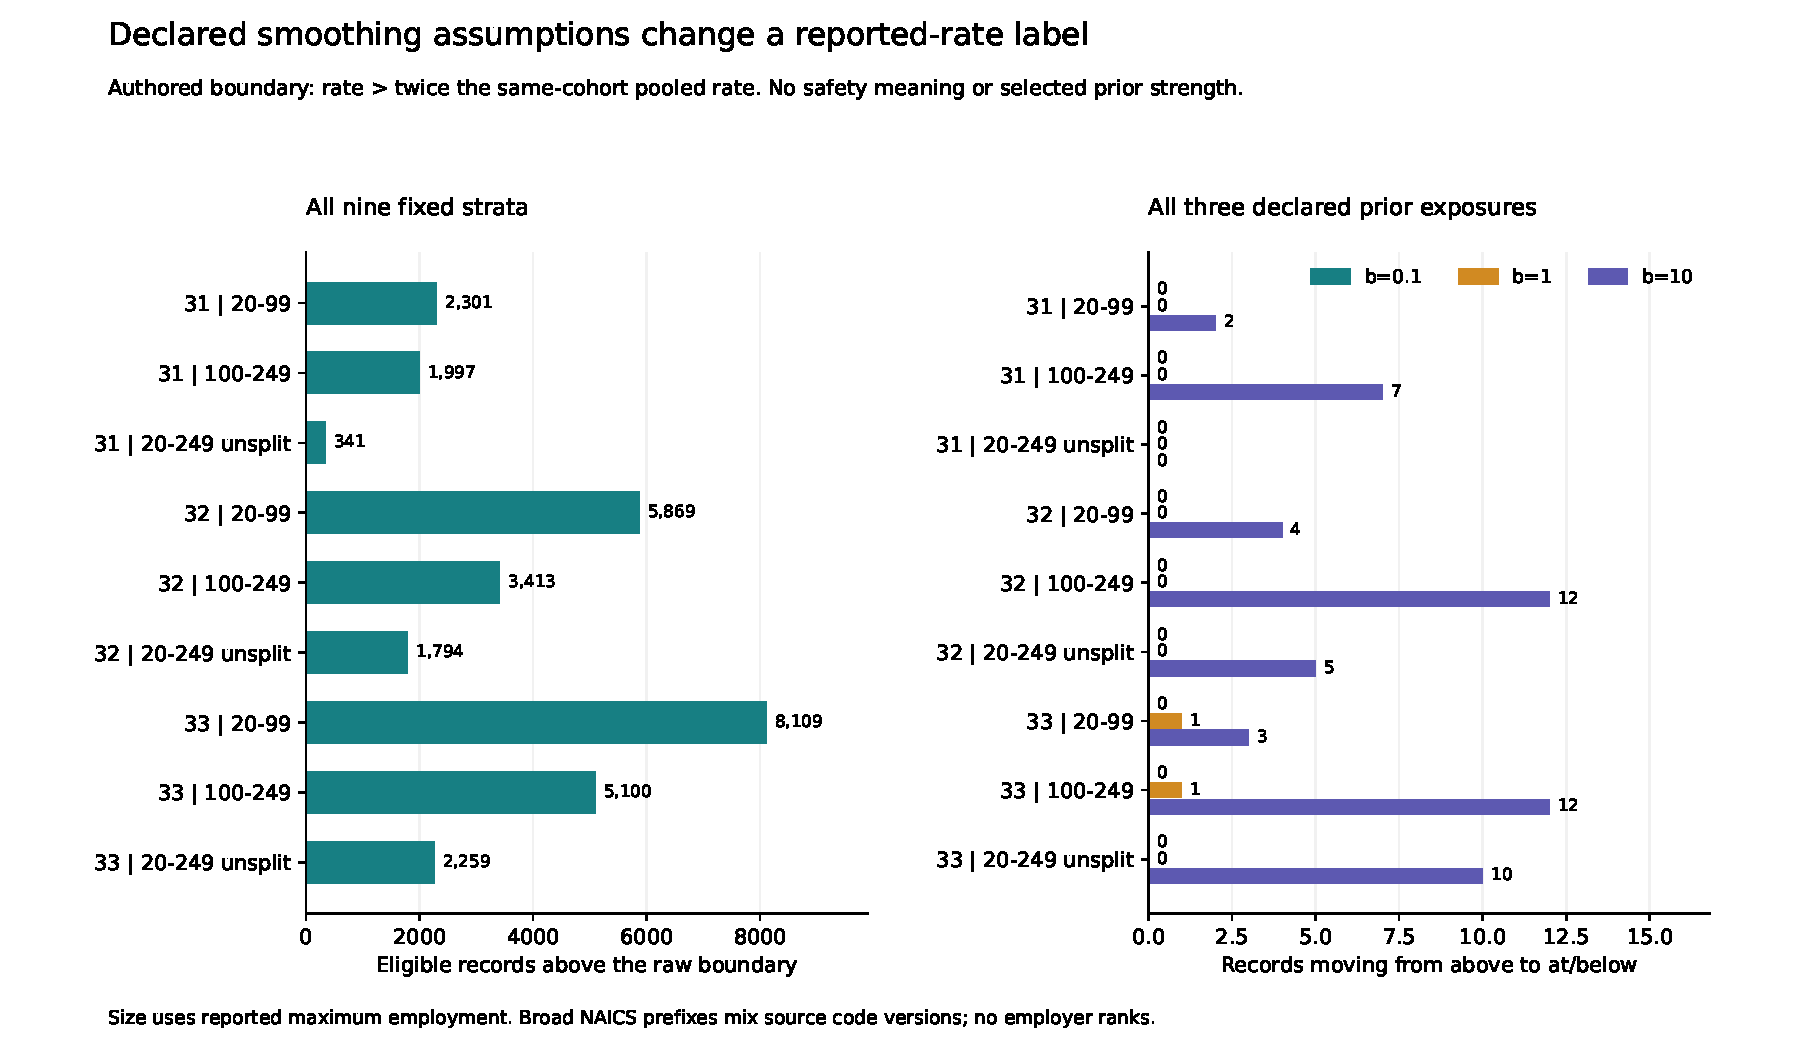
\includegraphics[width=9.4in,height=6.25in,keepaspectratio]{images/smoothing_sensitivity.pdf}\end{center}
\end{landscape}
\begin{landscape}
{\large\bfseries Complete source eligibility accounts\par}
\begin{center}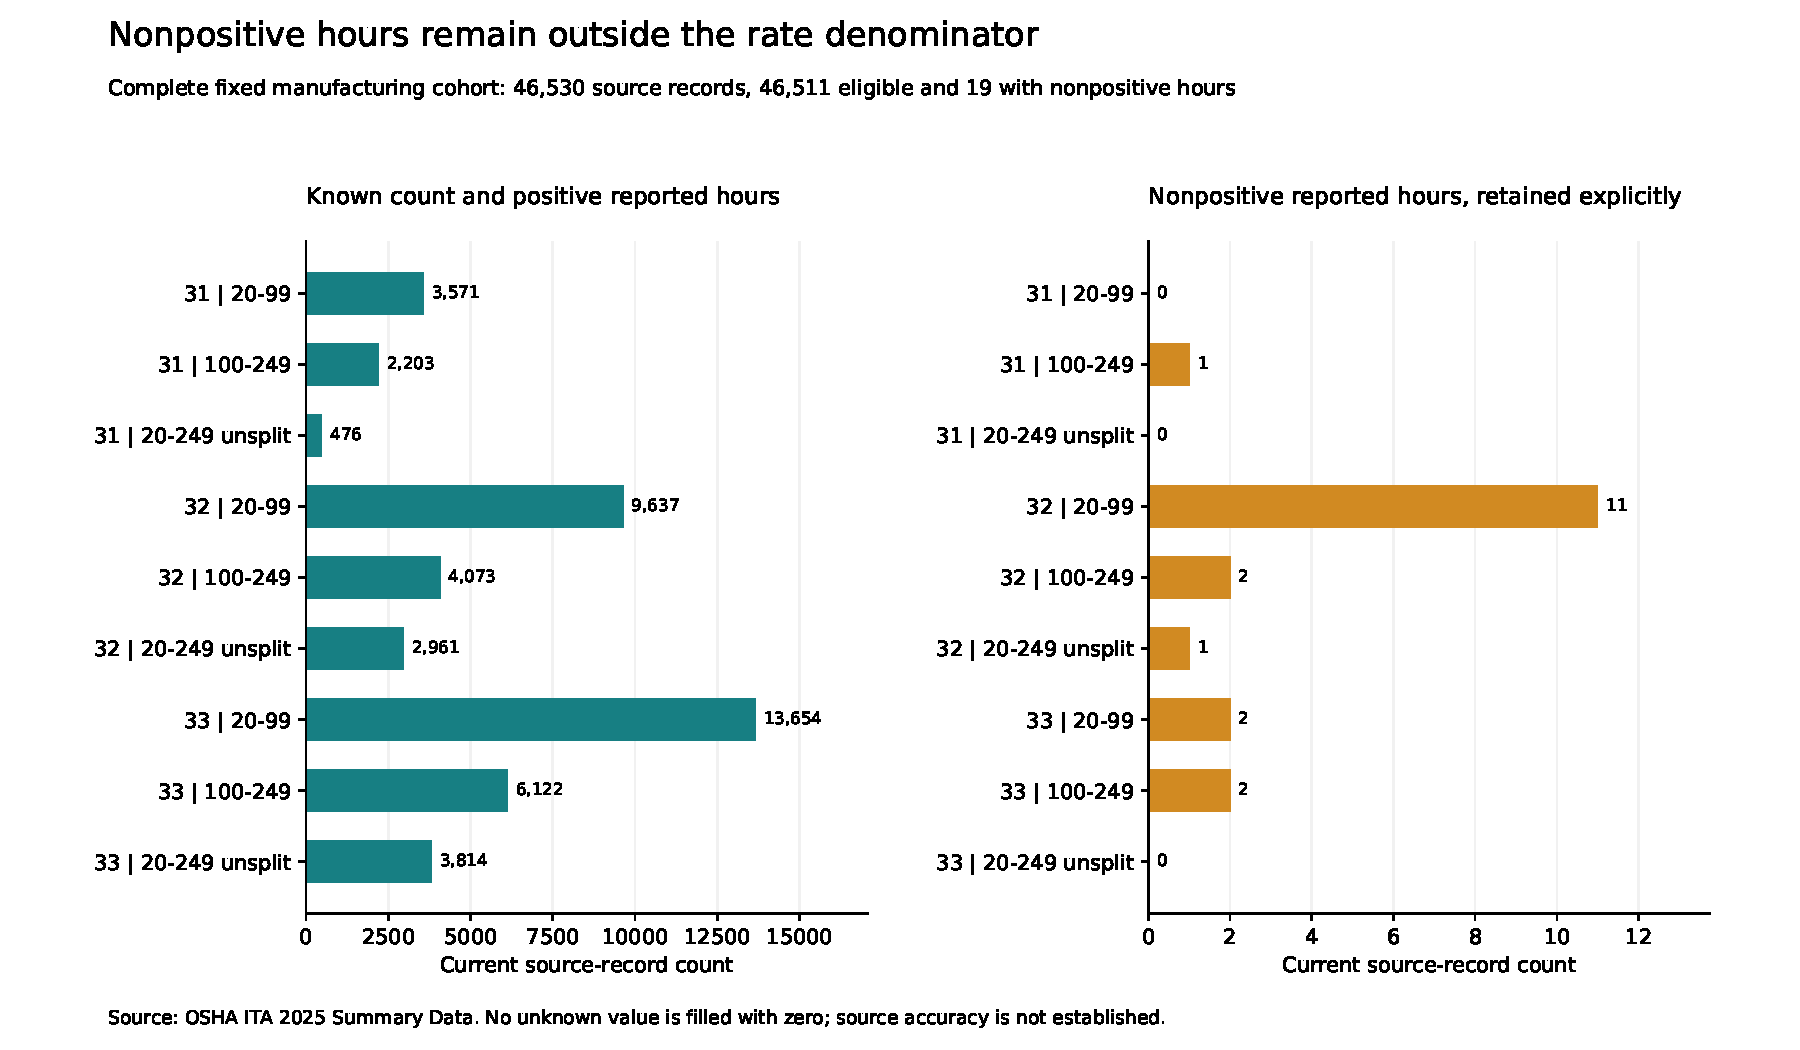
\includegraphics[width=9.4in,height=6.25in,keepaspectratio]{images/source_denominators.pdf}\end{center}
\end{landscape}
\end{document}
